\documentclass{zapiski}
\originfo{1}{}{}{2026}
\setcounter{page}{1}
\date{}

\usepackage[utf8]{inputenc}
\usepackage[T1]{fontenc}
\usepackage[english]{babel}

% The document is English throughout, so the Russian masthead of the class is
% suppressed and no Cyrillic encoding is loaded. This also removes the dependency
% on texlive-lang-cyrillic.
\renewcommand{\publnamef}{}
\renewcommand{\publnames}{}
\renewcommand{\russianvolinfo}{}

\usepackage{times}
\usepackage{url}
\usepackage{graphicx}
\usepackage{amssymb}
\usepackage[hidelinks]{hyperref}
\usepackage{booktabs}
\usepackage{caption}
\usepackage{cite}
\usepackage{array}
\usepackage{float}
\restylefloat{table}
\usepackage{tikz}
\usetikzlibrary{arrows.meta}
\definecolor{vbblue}{HTML}{2A78D6}
\definecolor{vbink}{HTML}{52514E}

\renewcommand{\UrlFont}{\ttfamily\small}

\english

\begin{document}

\title[The verifier bottleneck]{The Verifier Bottleneck: Can an AI Teach
Itself Mathematics?}

% =========================================================================
% AUTHORS. The venue does not anonymise submissions and requires the full list,
% every author registered on OpenReview and added to the submission, the mentor
% named, and a Contribution section.
%
% One author is filled in. Add the remaining co-authors below and give each of
% them a paragraph in the Contribution section, keeping the two lists in the
% same order.
% =========================================================================
\author[Churilkin et al.]{Artem Churilkin$^{1}$, Co-author Two$^{1}$,
Co-author Three$^{1}$}
\address[Artem Churilkin]{$^{1}$Affiliation}
\email{artem@superpositions.tech}

\begin{abstract}
This work studies whether low-rank fine-tuning on exact, automatically verified
composition trajectories can change the probability distribution of a small language
model so that correct programs take higher positions on new tasks under an unchanged
evaluation procedure. The experiments use Qwen3-0.6B~\cite{yang2025qwen3} in a
controlled environment of polynomial transformations over finite fields, where a
solution is a sequence of three atomic operations chosen from five. For every task all
125 distinct programs of depth three were enumerated and scored exactly, so the main
measure Hit@32 contains no sampler and no repeated candidates. Two branches of equal
training budget were compared, an atomic control and fine-tuning on verified
trajectories. Mean Hit@32 rose from 45.32 to 72.72 percent, a gain of 27.40 percentage
points with a 95 percent $t$ interval of $[25.40, 29.40]$ over six independent runs and
$p = 3.45 \times 10^{-7}$, positive in all six. A second series measured what the
surrounding pipeline contributes: structured exploration carries no advantage over
independent sampling at matched candidate diversity, and four hundred steps of training
with a verifiable reward change held-out coverage by $+0.22$ points. Transfer to
previously held local motifs was not confirmed in either series, and part of the atomic
skills degraded, so the positive effect should be read as reliable consolidation of
familiar families of compositions and transfer to new tasks, and not as the universal
emergence of an arbitrary new compositional ability.
\end{abstract}

\keywords{language model, skill composition, checking program, low-rank
fine-tuning, exact ranking, finite field, Hit@32, reproducible experiment}

\maketitle

\section{Introduction}
\label{sec:intro}

Modern language models can improve on formalisable tasks through cycles of generation,
automatic checking and further fine-tuning: the model forms several candidates, a
checking program picks out the correct ones, and those become new training material.
Schemes of this kind underlie self-taught reasoning, self-consistent inference,
step-level verification and training with a verifiable
reward~\cite{gulcehre2023rest,lightman2024verify,wang2023selfconsistency,zelikman2022star}.

The main question is what exactly changes after such training. In the first of two
possible effects the model only raises the probability of solutions already available
to it but rare; in the second it begins to reproduce compositions of actions on new
tasks whose input states were absent from the training set. Distinguishing these
regimes matters for the theory of self-improvement and for the design of practical
systems of mathematical inference~\cite{liu2025prorl,yue2025rl}.

The project considers two control axes: the informativeness of the checking program,
and the availability of diverse candidates together with the possibility of combining
learned skills. Early experiments showed that an external widening of the search is
easily confused with a real change in the parameters. The evaluation procedure is
therefore fixed and never changed between the compared branches: for every task the
same complete set of programs is built, and the model influences only their probability
order. The aim is to test whether low-rank fine-tuning on exact, automatically verified
composition trajectories raises the rank of correct programs on new tasks against
additional atomic training of the same budget. A positive result raises a second
question that experiment cannot answer, namely how much of the effect belongs to the
fine-tuning and how much to the surrounding pipeline of search and reward, which
Section~\ref{sec:second} measures.

The contributions are four measurements. Fine-tuning on verified composition
trajectories raises exact ranking of correct depth-3 programs by 27.40 percentage
points against an atomic control of equal budget, 95 percent $t$ interval
$[25.40, 29.40]$, positive in all six independent runs, carrying to new finite fields
at 26.13 points. The advantage of structured exploration over independent sampling is
accounted for by the number of distinct programs the search actually tries: at matched
diversity it is $-1.11$ points, interval $[-4.22, +1.89]$. Four hundred steps of
policy-gradient training with an exact binary reward leave held-out coverage unchanged
within three percentage points, at $+0.22$, while at the arm where the preferences of
the policy dominate the same runs make it 2.37 times more accurate per candidate and
2.10 times narrower. Supervision does not transfer to adjacent operation pairs withheld
from it, at $-16.02$ and $-11.80$ points here and at $-13.47$ and $-15.07$ in the
second series, where a control shows that adapters whose data contained those pairs
reach Hit@32 of 0.935 and 0.933 on exactly the families that the withheld adapters
fail.

\section{Related Work}
\label{sec:related}

Self-training with automatic checking has four steps: the model forms candidates, an
external algorithm checks each of them, the correct ones are stored as positive
trajectories, and the parameters are updated so that their probability grows. Zelikman
et al.~\cite{zelikman2022star} bootstrap reasoning traces this way, Wang et
al.~\cite{wang2023selfconsistency} aggregate over sampled traces, Lightman et
al.~\cite{lightman2024verify} supervise the individual steps, and Gulcehre et
al.~\cite{gulcehre2023rest} formalise the loop as repeated growth and improvement
stages. The reliability of the checking program is described by $\alpha$, the
probability of accepting a correct answer, and $\beta$, the probability of accepting an
incorrect one: at $\alpha > \beta$ the signal carries information about correctness, at
$\alpha = \beta$ it is uninformative, and at $\alpha < \beta$ it directs training in the
wrong direction~\cite{cover2006information}.

Whether such training expands ability or concentrates it is contested. Yue et
al.~\cite{yue2025rl} report that a verifiable reward raises single-sample accuracy
while leaving coverage at large $K$ at or below the base model, and
ProRL~\cite{liu2025prorl} reports the opposite under a much longer schedule. Both
measure coverage by sampling, so the number of distinct candidates a sampler happens to
produce enters the measurement; structured search is a second way to raise that
number~\cite{yao2023tot}. This work removes the sampling term by scoring the complete
candidate space and measures the contribution of structure against a baseline matched
on diversity.

Compositional generalisation means combining mastered transformations into a sequential
program. Separate command of $A$ and $B$ does not guarantee correct execution of $A$
after $B$: order changes the result and an early error propagates. Lake and
Baroni~\cite{lake2018systematicity} show that sequence models generalise poorly to
held-out combinations of familiar primitives, Zhao et al.~\cite{zhao2024skill} study
whether skill composition can be learned from examples, and Dziri et
al.~\cite{dziri2023faith} trace compositional failures to the structure of the task
graph. This work uses the discover-and-distill scheme: exhaustive enumeration and an
exact checking program determine the correct trajectories, and the model is fine-tuned
on them with a low-rank adapter~\cite{hu2022lora}, receiving the full target answer
including the operations and the verifiable intermediate states. Training a model on
its own outputs can degrade it~\cite{shumailov2024collapse}; the loop here is protected
by construction, since an exact checking program admits only correct trajectories.

\section{Environment and data}
\label{sec:env}

The state is a polynomial of degree at most $d$ over the finite field $F_p$, stored as
the vector of its coefficients $[c_0, \ldots, c_d]$ taken modulo $p$, with the length
preserved including leading zeros. Five exact atomic operations are defined over this
state: SH1 shifts the argument by one, SC2 scales it by two, REV reverses the
coefficient vector, and AC1 and AX1 add one to the free coefficient and to the
coefficient at $x$. All are computed deterministically, do not increase the size of the
state and admit exhaustive enumeration of programs of small depth
(Table~\ref{tab:ops}).

The frozen protocol of the project fixes the rest of the environment for both
series. Training uses the fields 5, 7, 13, 19, 23 and 29, the fields 11 and 17 are
held back for transfer, and three \emph{motifs} are held back from supervision, a
motif being an adjacent ordered pair of operations. The three are AX1 followed by
SH1, AC1 followed by REV, and SC2 followed by AX1. At depth two the space contains
$5^2 = 25$ programs, at depth three 125, and at depth four 625.
Appendix~\ref{app:examples} works through one program of each depth and gives a
target that two different programs reach.

In PLAN mode the model receives the field, the start and target vectors, the list of
admissible operations and the fixed program length, and must return a sequence of
operations; in APPLY mode it is given an explicit sequence and must compute the final
vector. APPLY was used to control the preservation of atomic skills, and the main
compositional result was measured in PLAN mode.

The training set of the confirmatory series included 4000 composition tasks, and the
final sets were generated separately, frozen before the series and not used when
selecting hyper-parameters. Four families separate different kinds of transfer: A tests
new input states under familiar compositional signatures and familiar fields, B holds
local motifs under familiar fields, C uses familiar signatures in new fields, and D
combines the two, with 1000 tasks each in A and B and 500 each in C and D.
Appendix~\ref{app:prereg} gives their structure and the integrity checks.

\section{Method}
\label{sec:method}

\subsection{Compared branches}

Each independent run started from one frozen atomic adapter and split into two branches
of equal budget. The main branch received full correct composition trajectories and 20
percent atomic replay; the control branch received an equal number of training tokens
and steps on atomic tasks alone, so a difference in the result cannot be explained by a
longer period of training. Both branches used low-rank adaptation with identical
settings and identical base weights, and new adapters were created for each run.
Figure~\ref{fig:design} and Table~\ref{tab:hyper} in Appendix~\ref{app:prereg} state
the design and the settings.

\subsection{Exact ranking and metrics}

The evaluation did not use random generation and did not depend on random repetitions
of one and the same program. For every task all distinct programs of the fixed depth
were enumerated. The model score of a program is the sum of the conditional logarithms
of the probabilities of its actions,
\begin{equation}
L(o_1, \ldots, o_d \mid x) = \sum_{i=1}^{d} \log p_\theta\!\left(o_i \mid x, o_1,
\ldots, o_{i-1}\right).
\label{eq:score}
\end{equation}
Programs were sorted by decreasing score, ties were broken by the lexicographic order
of the operation signatures, and the checking program marked all correct variants. The
main measure Hit@32 is the share of tasks for which at least one correct program enters
the first 32 positions. Unlike random pass@$K$~\cite{chen2021codex} it does not depend
on the repeated generation of identical strings. Depth two has only 25 candidate
programs, so Hit@32 is structurally saturated there and a zero difference on it carries
no information about the absence of an effect.

\subsection{Statistical plan}

The independent unit of confirmation was the training run: a thousand tasks inside one
run are not a thousand independent models. For each of the six runs the difference in
Hit@32 between the branches was computed on the same 1000 tasks of family A, and over
the six differences the mean, the 95 percent $t$ interval and the two-sided one-sample
$t$ test were computed. An exact sign-permutation test over all $2^6 = 64$ sign
combinations and a two-level resampling over both runs and tasks served as robustness
checks, and the Holm correction was applied to five secondary
measures~\cite{efron1993bootstrap,holm1979procedure}. The conditions for a positive
result were fixed before the final set was opened; Appendix~\ref{app:prereg} gives them
with the resampling detail.

\section{Results}
\label{sec:results}

\subsection{Main confirmatory result}

The starting atomic adapter reached 99.8 percent in PLAN mode and 91.5 percent in
APPLY mode, its weakest atomic operation being the shift SH1 at 57.5 percent.

On the main set A of depth three the control branch solved on average 45.32 percent of
the tasks on Hit@32, and after fine-tuning on verified composition trajectories the
mean was 72.72 percent. The absolute gain equals 27.40 percentage points, a factor of
1.60 in the share of successfully ranked tasks. The 95 percent $t$ interval over the
six independent runs equals $[25.403, 29.397]$ percentage points and the two-sided $p$
value of the one-sample $t$ test equals $3.445 \times 10^{-7}$. All six runs gave a
positive difference, the exact sign-permutation test gave $p = 0.03125$, and the
two-level resampling gave the wider interval $[23.117, 31.667]$. Both intervals lie
entirely above the preregistered threshold of no effect, and all preregistered
conditions of a positive result were met.Figure~\ref{fig:perrun} shows the individual runs.

\begin{figure}[!tbh]
    \centering
    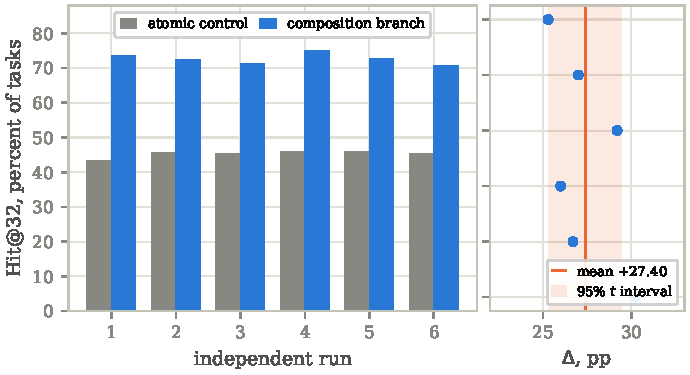
\includegraphics[width=0.74\textwidth]{pic/fig3_per_run.pdf}
    \caption{Left, Hit@32 of the two branches in each of the six independent runs, on
    the same 1000 tasks of family A at depth three. Right, the six per-run
    differences, the mean of 27.40 percentage points and the 95 percent $t$ interval
    computed over them. The spread runs from 25.3 to 30.2 percentage points.}
    \label{fig:perrun}
\end{figure}

The effect appeared in a continuous measure as well. In all six runs the normalised
probability mass of the correct set grew, by 4.41 percentage points on average with
a 95 percent $t$ interval of $[4.25, 4.57]$. The model therefore did not merely move
a single program across the boundary at position 32.

\subsection{Boundaries of transfer}

The secondary sets determine the boundaries of the effect, and
Figure~\ref{fig:transfer} in Appendix~\ref{app:integrity} collects them. On family C,
where the composition families stayed familiar but new finite fields were used, the
gain was 26.13 percentage points, positive in all six runs, which confirms transfer of
the mastered compositional regularities to new arithmetic fields and shows that
training did not reduce to memorising specific coefficients or a specific modulus. On
family B with local motifs held back in advance the result fell by 16.02 points, and on
family D, which combined held motifs and new fields, by 11.80. Fine-tuning therefore
consolidated familiar families of composition trajectories and did not form a universal
rule for motifs completely excluded from the training data. On the combined set of
depth four a positive gain of 5.20 points was obtained. After the Holm correction the
three depth-3 rows and the depth-4 row have $p$ values of $8.487 \times 10^{-5}$,
$1.879 \times 10^{-7}$, $1.024 \times 10^{-5}$ and $2.976 \times 10^{-5}$.

\subsection{Preservation of atomic skills}

The positive compositional result was accompanied by partial forgetting. After the
control atomic training the mean PLAN was 99.72 percent and the mean APPLY 90.28; after
composition fine-tuning PLAN was 97.78 and APPLY 85.70. The main contribution came from
SH1, which the control branch left at 51.5 percent and the composition branch at 29.08,
while the remaining four operations stayed at 99 to 100 percent, and only two of the twelve trained
branch-and-run pairs met the descriptive forgetting threshold of two percentage points.
In the final preregistration atomic forgetting was defined as descriptive and not
blocking, and an earlier exploratory pilot on the configuration this series froze
remains formally negative under its own older atomic-forgetting gate.

\subsection{What the surrounding pipeline contributes}
\label{sec:second}

A second series, on the same base model and the same field division but with its own
independently generated splits, three training seeds, 300-task evaluation sets for the
depth and field grid and 250-task sets for the motif families, and its own shared
atomic checkpoint as the reference that every gain below is measured against,
measures the contribution of the search and the reward around the fine-tuning. Its
numbers are not comparable with the intervals above, because it uses a different
unit of replication and a crossed seed-by-task bootstrap.
Figure~\ref{fig:contrasts} collects its contrasts, and Appendix~\ref{app:second}
gives the tables.

Three of its measurements bound the reading of the first series. The advantage of
structured exploration over independent sampling, reported by an earlier pilot at 16.0
percentage points and reproduced at 16.33, becomes $-1.11$ points with an interval of
$[-4.22, +1.89]$ once the baseline is tempered to the diversity that structured search
realises. Policy-gradient training~\cite{shao2024deepseekmath} at the exploration
optimum changes held-out coverage after 400 steps by $+0.22$ points, interval
$[-3.11, +3.67]$, while raising per-candidate accuracy from 0.0151 to 0.0358 and
lowering distinct programs per task from 3.80 to 1.81, a redistribution of probability
inside the existing support. Direct supervision reproduces the confirmatory result at
48.22 and 59.11 points while an equal-budget atomic control, trained on an atomic pool that
covers the fields 5 and 7 alone, moves the same measurement by $+0.11$ and $+1.67$ with
both intervals containing zero; that study's own registered
retention rule does not count the gain as a success, because the adapters that produce
it lose the APPLY mode entirely, and the motif axis
reproduces at $-13.47$ and $-15.07$ points with a motif main effect of $+71.27$ against
a field main effect of $-1.00$. Adapters whose data contained the three withheld pairs
reach Hit@32 of 0.935 and 0.933 on exactly those families, so the failure follows from
the absence of the pair from supervision and not from a property of the tasks, and the
contrast is sharp: the fields 11 and 17 are absent from every training file in the same
sense and cost one point, while the withheld pairs cost 71.
Appendix~\ref{app:second} gives the tables and the registered status of each study.

\section{Discussion}
\label{sec:discussion}

The main result shows that full verified composition trajectories can be transferred
into the parameters of a small language model. Under an unchanged evaluation procedure
the correct programs moved upward in the complete ranked space, so the effect cannot be
explained by a wider search, by the removal of repetitions or by more candidates during
checking. The control branch received the same budget on fresh atomic tasks, so the
difference of 27.40 percentage points reflects the information content of the
composition trajectories and not an additional number of optimiser steps, and the
equal-budget control of the second series measures the same thing on independently
generated data. Family A contains new states and tasks under familiar signatures and
familiar fields, so the result should be called a transfer of verified trajectories to
new inputs, and not a proof of the mastery of an arbitrary previously unseen
composition. The negative results on B and D show that local motifs excluded in advance
were not derived automatically from the separate atomic skills.

The improvement was accompanied by a deterioration in part of the atomic skills, which
agrees with the known problem of catastrophic forgetting under sequential
fine-tuning~\cite{kirkpatrick2017forgetting}, and 20 percent atomic replay did not
ensure the full preservation of SH1. Two statements have to be separated: the positive
compositional result is statistically confirmed in the preregistered main check, and
the final model is at the same time not unconditionally better on all skills. Taken
together with the degraded-verifier levels of Appendix~\ref{app:second}, the second
series locates the constraint of the setting: a checking program that accepts every
correct trajectory and rejects every incorrect one does not let policy-gradient
training expand the set of reachable programs, and one corrupted at one label in two
still permits direct supervision to stand 41 points above the untrained baseline. In this
environment the binding constraint lies on the side of generation, and the unit in
which the reachable set grows is the adjacent pair of operations that supervision
demonstrates.

\subsection{Limitations}

The study uses one architecture and one model size, and transfer to other models
requires separate verification. The main positive result concerns familiar families of
compositional signatures on new inputs; transfer to held local motifs is not confirmed,
and three motifs were withheld out of the 25 adjacent pairs. Atomic forgetting was
substantial, especially for SH1. Six independent runs are sufficient for the criteria
fixed in advance, and the exact sign-permutation test has a coarse resolution at that
number. The environment is synthetic: its advantage is exact checking and complete
enumeration. Appendix~\ref{app:limits} gives the full list.

\section{Conclusion}
\label{sec:conclusion}

A preregistered confirmatory experiment on the transfer of verified composition
trajectories into the parameters of a small language model was carried out, using
Qwen3-0.6B, a controlled environment of polynomial transformations over finite fields,
an exact checking program and the complete ranking of all programs of a fixed depth.
The main hypothesis is confirmed: on 1000 new tasks of family A the mean Hit@32 after
composition fine-tuning was 72.72 percent against 45.32 in the control branch of equal
budget, a gain of 27.40 percentage points with a 95 percent $t$ interval of
$[25.403, 29.397]$ and $p = 3.445 \times 10^{-7}$, positive in all six runs, with
transfer to new finite fields at 26.13 points. Transfer to local motifs held back in
advance is not confirmed, which bounds the domain of the conclusion and shows that the
mastery of familiar composition families is not identical to universal compositional
generalisation. The second series adds that structured exploration carries no advantage
at matched diversity, that four hundred steps with an exact reward sharpen the policy
by 2.37 times per candidate and narrow it by 2.10 while leaving coverage unchanged
within three points, and that an equal-budget atomic control moves the composition
measure by 0.11 and 1.67 points. Exact verified composition trajectories can therefore
be consolidated in the parameters of a small language model and can substantially raise
the rank of correct programs on new tasks under an unchanged evaluation procedure; what
bounds the result in this environment is the set of programs the model can produce at
all.

\section{Contribution}
\label{sec:contribution}

% ---------------------------------------------------------------------------
% FILL IN BEFORE SUBMISSION. The venue requires a statement of what each team
% member contributed. The four blocks below are the work split the project
% actually planned, taken from its own internal specification; assign the real
% names and adjust to what each person did.
% ---------------------------------------------------------------------------

\textbf{Artem Churilkin} proposed and implemented the measurement the paper is built
on: the exhaustive enumeration of every program of a given depth, the selection of the
correct ones by the exact checking program, and the ranking metric built on them, which
asks whether fine-tuning placed those programs higher and not whether a sampler
happened to find them. He ran the fine-tuning on full correct trajectories and the
control training on known-correct solutions, which separates whether the model can
represent these compositions from whether a given method finds them; designed the
decomposition that varies program depth and finite field on separate axes instead of
both at once; and ran the final comparison of methods at an equal candidate budget
across several seeds. He wrote the manuscript.

\textbf{Co-author Two} REPLACE THIS WITH YOUR OWN CONTRIBUTION.

\textbf{Co-author Three} REPLACE THIS WITH YOUR OWN CONTRIBUTION.

All authors agreed on the claims the paper makes, on the boundary between what the
experiments establish and what they do not, and on the retention of the negative
results in full.

\section*{Acknowledgments}

We thank our mentor \textbf{Serguei Barannikov} for the problem statement and for the
protocol behind this study, carried out within SMILES 2026.

\clearpage
\appendix
\renewcommand{\thesection}{\Alph{section}}
\setcounter{section}{0}

\section{Worked examples of the environment}
\label{app:examples}

Table~\ref{tab:opsexample} shows all five transformations on one starting polynomial
over $F_{11}$, which makes it visible that they change different parts of the state.
Figure~\ref{fig:example} traces one shortest program of depth three and gives one
target reached by two different programs of depth four.
Table~\ref{tab:examples} collects further correct compositions across fields, degrees
and depths. Every row was re-executed with the deterministic interpreter of the
experiments, and every uniqueness claim was re-checked by exhaustive search over all
programs of that depth and shorter.

\begin{table}[!tbh]
\centering\footnotesize\setlength{\tabcolsep}{4pt}
\begin{tabular}{|l|l|p{.34\linewidth}|}
\hline
\textbf{Code} & \textbf{Transformation} & \textbf{Effect} \\
\hline
SH1 & $P(x) \mapsto P(x+1)$ & shift of the argument by one \\ \hline
SC2 & $P(x) \mapsto P(2x)$ & scaling of the argument \\ \hline
REV & $[c_0, \ldots, c_d] \mapsto [c_d, \ldots, c_0]$ & reversal of the vector \\ \hline
AC1 & $c_0 \mapsto c_0 + 1$ & change of the free coefficient \\ \hline
AX1 & $c_1 \mapsto c_1 + 1$ & change of the coefficient at $x$ \\ \hline
\end{tabular}
\caption{The five atomic transformations, all taken modulo $p$. Each one is
computed deterministically and none of them changes the length of the state
vector, so programs of small depth can be enumerated in full. AC1 and AX1 look
similar and touch different coordinates, so after REV or SH1 they lead to
different final states.}
\label{tab:ops}
\end{table}

% ------------------------------------------------- worked example, one polynomial
\begin{table}[!tbh]
\centering\scriptsize\setlength{\tabcolsep}{4pt}
\begin{tabular}{|l|p{.50\linewidth}|l|}
\hline
\textbf{Code} & \textbf{Exact action on $P(x) = 2 + 5x + 3x^2 + 4x^3$} & \textbf{Result} \\
\hline
SH1 & shift of the argument, $P(x) \to P(x+1)$: $2 + 5(x+1) + 3(x+1)^2 + 4(x+1)^3 = 14 + 23x + 15x^2 + 4x^3$ & $[3, 1, 4, 4]$ \\ \hline
SC2 & scale of the argument, $P(x) \to P(2x)$: the coefficient at $x^i$ is multiplied by $2^i$, giving $[2, 10, 12, 32]$ & $[2, 10, 1, 10]$ \\ \hline
REV & reversal of the coefficient vector. This is neither a reversal of digits nor a substitution of $-x$ for $x$: $[c_0, c_1, c_2, c_3] \to [c_3, c_2, c_1, c_0]$ & $[4, 3, 5, 2]$ \\ \hline
AC1 & one is added to the free coefficient only: $[2+1, 5, 3, 4]$ & $[3, 5, 3, 4]$ \\ \hline
AX1 & one is added to the coefficient at $x$ only: $[2, 5+1, 3, 4]$ & $[2, 6, 3, 4]$ \\ \hline
\end{tabular}
\caption{All five transformations on one starting polynomial over $F_{11}$, with the
state $[2, 5, 3, 4]$. Coefficients are reduced modulo 11 after every operation. AC1
and AX1 look similar and change different coordinates, so after REV or
SH1 they lead to different final states. Every row was re-executed with the same
deterministic interpreter that the experiments use.}
\label{tab:opsexample}
\end{table}


\begin{figure}[!tbh]
\centering
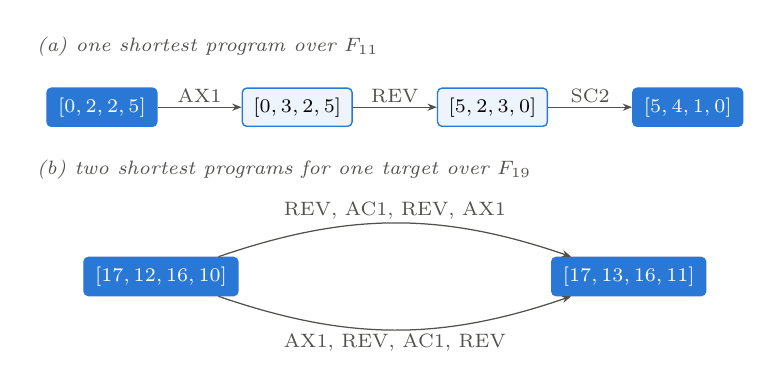
\begin{tikzpicture}[
  x=1cm, y=1cm,
  state/.style      = {rectangle, rounded corners=1.6pt, draw=vbblue,
                       line width=0.5pt, inner xsep=4pt, inner ysep=3.4pt,
                       fill=vbblue!8, font=\scriptsize},
  anchorstate/.style= {state, fill=vbblue, text=white, draw=vbblue},
  flow/.style       = {-{Stealth[length=3.4pt,width=2.6pt]}, draw=vbink,
                       line width=0.45pt},
  op/.style         = {font=\scriptsize, inner sep=1.6pt, text=vbink,
                       fill=white, inner ysep=1pt},
  lab/.style        = {font=\scriptsize\itshape, text=vbink, anchor=west},
]
\node[lab] at (-0.15,2.62) {(a) one shortest program over $F_{11}$};
\node[anchorstate] (a0) at (0.80,1.85) {$[0,2,2,5]$};
\node[state]       (a1) at (3.28,1.85) {$[0,3,2,5]$};
\node[state]       (a2) at (5.76,1.85) {$[5,2,3,0]$};
\node[anchorstate] (a3) at (8.24,1.85) {$[5,4,1,0]$};
\draw[flow] (a0) -- node[op, above=0.4pt]{AX1} (a1);
\draw[flow] (a1) -- node[op, above=0.4pt]{REV} (a2);
\draw[flow] (a2) -- node[op, above=0.4pt]{SC2} (a3);
\node[lab] at (-0.15,1.06) {(b) two shortest programs for one target over $F_{19}$};
\node[anchorstate] (b0) at (1.55,-0.30) {$[17,12,16,10]$};
\node[anchorstate] (b1) at (7.49,-0.30) {$[17,13,16,11]$};
\draw[flow] (b0) to[out=19,in=161]
  node[op, midway, above=0.2pt]{REV, AC1, REV, AX1} (b1);
\draw[flow] (b0) to[out=-19,in=-161]
  node[op, midway, below=0.2pt]{AX1, REV, AC1, REV} (b1);
\end{tikzpicture}
\caption{Panel (a) gives every intermediate state of one shortest program of depth
three over $F_{11}$. Order matters: exchanging the first two operations sends the
start to $[5,6,8,0]$ instead of the target. Panel (b) gives one target over $F_{19}$
that two different programs of depth four reach. Because several programs may reach
one target, Hit@32 uses the best rank among all correct programs.}
\label{fig:example}
\end{figure}

% ------------------------------------------------- diverse compositions
\begin{table}[!tbh]
\centering\scriptsize\setlength{\tabcolsep}{3pt}
\begin{tabular}{|c|c|l|l|l|l|}
\hline
\textbf{Depth} & \textbf{$p$} & \textbf{Start} & \textbf{Target} & \textbf{A correct program} & \textbf{Type} \\
\hline
2 & 7  & $[1, 2, 3]$        & $[3, 2, 2]$        & AC1, REV           & unique shortest \\ \hline
3 & 11 & $[0, 2, 2, 5]$     & $[5, 4, 1, 0]$     & AX1, REV, SC2      & unique shortest \\ \hline
3 & 7  & $[4, 4, 5, 6]$     & $[0, 2, 4, 5]$     & SH1, REV, AC1      & unique shortest \\ \hline
4 & 11 & $[10, 10, 2]$      & $[0, 10, 7]$       & SC2, REV, SC2, SH1 & unique shortest \\ \hline
4 & 23 & $[7, 8, 18, 5]$    & $[16, 20, 1, 10]$  & REV, AX1, SH1, SC2 & one solution \\ \hline
4 & 19 & $[17, 12, 16, 10]$ & $[17, 13, 16, 11]$ & the two of Fig.~\ref{fig:example} & two solutions \\ \hline
\end{tabular}
\caption{Correct compositions across different fields, degrees and depths. Every
row was re-executed with the deterministic interpreter of the experiments, and
every uniqueness claim was re-checked by exhaustive search over all programs of
that depth and shorter. Order matters throughout: on the second row the sequence
REV, AX1, SC2 gives $[5, 6, 8, 0]$ instead of the target, and on the fourth row
exchanging the first two operations gives $[4, 8, 6]$.}
\label{tab:examples}
\end{table}


\section{Design, preregistration and statistical detail}
\label{app:prereg}

\begin{figure}[!tbh]
\centering
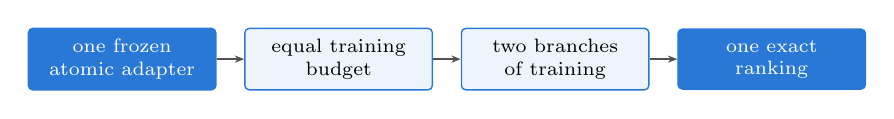
\begin{tikzpicture}[
  x=1cm, y=1cm,
  stage/.style = {rectangle, rounded corners=1.6pt, draw=vbblue, line width=0.5pt,
                  fill=vbblue!8, font=\scriptsize, align=center,
                  inner xsep=4pt, inner ysep=4pt, text width=2.1cm},
  head/.style  = {stage, fill=vbblue, text=white},
  flow/.style  = {-{Stealth[length=3.4pt,width=2.6pt]}, draw=vbink, line width=0.45pt},
]
\node[head]  (s1) at (0.00,0) {one frozen\\atomic adapter};
\node[stage] (s2) at (2.75,0) {equal training\\budget};
\node[stage] (s3) at (5.50,0) {two branches\\of training};
\node[head]  (s4) at (8.25,0) {one exact\\ranking};
\draw[flow] (s1) -- (s2);
\draw[flow] (s2) -- (s3);
\draw[flow] (s3) -- (s4);
\end{tikzpicture}
\caption{The logic of the confirmatory experiment. Every independent run starts from
one and the same frozen atomic adapter, the two branches receive an identical number
of optimiser steps, epochs, training tokens and an identical effective batch size,
and both are then evaluated by one and the same exhaustive ranking. Only the type of
training material differs between the branches.}
\label{fig:design}
\end{figure}

% ------------------------------------------------- final sets
\begin{table}[!tbh]
\centering\footnotesize\setlength{\tabcolsep}{5pt}
\begin{tabular}{|c|l|l|r|l|}
\hline
\textbf{Set} & \textbf{Signatures} & \textbf{Fields} & \textbf{Tasks} & \textbf{Role} \\
\hline
A & familiar & familiar & 1000 & main test \\ \hline
B & held motifs & familiar & 1000 & transfer to new motifs \\ \hline
C & familiar & new & 500 & transfer between fields \\ \hline
D & held motifs & new & 500 & double transfer \\ \hline
\end{tabular}
\caption{Structure of the final sets of the confirmatory series. All specific input
states and tasks were new, the sets were frozen before the confirmatory series and
were not used to select any hyper-parameter, and the leak audit found no
intersection with the atomic, training and development sets. Check sets of 125
tasks at depths 2 and 4 were built for each family in addition.}
\label{tab:sets}
\end{table}

% ------------------------------------------------- success conditions
\begin{table}[!tbh]
\centering\footnotesize\setlength{\tabcolsep}{6pt}
\begin{tabular}{|p{.46\linewidth}|l|}
\hline
\textbf{Condition} & \textbf{Threshold} \\
\hline
mean gain in Hit@32 & at least 5 percentage points \\ \hline
lower bound of the 95 percent $t$ interval & strictly above zero \\ \hline
two-sided $p$ value & below 0.05 \\ \hline
number of positive runs & at least 5 of 6 \\ \hline
data integrity & full check, equal budget, no leaks \\ \hline
\end{tabular}
\caption{Conditions for a positive result, fixed before the final set was opened,
together with the main endpoint, the set A, the depth and the number of independent
runs. All five were met.}
\label{tab:conditions}
\end{table}

% ------------------------------------------------- branches
\begin{table}[!tbh]
\centering\footnotesize\setlength{\tabcolsep}{5pt}
\begin{tabular}{|l|p{.30\linewidth}|p{.34\linewidth}|}
\hline
\textbf{Branch} & \textbf{Training data} & \textbf{Purpose} \\
\hline
atomic control & fresh atomic tasks & control for the effect of further training and of the number of tokens \\ \hline
composition branch & full correct composition trajectories and 20 percent atomic replay & consolidation of verified operation sequences \\ \hline
\end{tabular}
\caption{The two branches of the confirmatory series. Each independent run started
from one frozen atomic adapter and split into these two. The correct composition
trajectories were found by exhaustive search and confirmed by the deterministic
verifier. The main branch received all the tokens of the program and the
intermediate states, and the control branch received an equal number of training
tokens and steps on atomic tasks alone, so a difference in the result cannot be
explained by a longer period of training.}
\label{tab:branches}
\end{table}

% ------------------------------------------------- hyper-parameters
\begin{table}[!tbh]
\centering\footnotesize\setlength{\tabcolsep}{6pt}
\begin{tabular}{|l|r|}
\hline
\textbf{Parameter} & \textbf{Value} \\
\hline
LoRA rank & 32 \\ \hline
scaling factor & 64 \\ \hline
dropout probability & 0.05 \\ \hline
learning rate & $1 \times 10^{-4}$ \\ \hline
epochs & 2 \\ \hline
effective batch size & 64 \\ \hline
warm-up fraction & 3 percent \\ \hline
gradient-norm clip & 1.0 \\ \hline
arithmetic format & bfloat16 \\ \hline
atomic replay in the main branch & 20 percent \\ \hline
\end{tabular}
\caption{Fine-tuning parameters of the confirmatory series, from its frozen protocol.
Both branches used low-rank adaptation with these settings and the base weights
stayed identical, and new adapters were created for every independent run so that
stability across runs could be assessed.}
\label{tab:hyper}
\end{table}

% ------------------------------------------------- statistical confirmation
\begin{table}[!tbh]
\centering\footnotesize\setlength{\tabcolsep}{6pt}
\begin{tabular}{|l|r|}
\hline
\textbf{Quantity} & \textbf{Value} \\
\hline
mean gain & $+27.40$ pp \\ \hline
95 percent $t$ interval & $[25.403, 29.397]$ pp \\ \hline
$t$, degrees of freedom & 35.275, $\mathrm{df} = 5$ \\ \hline
two-sided $p$ from the $t$ test & $3.445 \times 10^{-7}$ \\ \hline
positive runs & 6 of 6 \\ \hline
exact sign-permutation test & $p = 0.03125$ \\ \hline
two-level bootstrap 95 percent interval & $[23.117, 31.667]$ pp \\ \hline
\end{tabular}
\caption{Statistical confirmation of the main effect on set A at depth 3. The unit
of replication is the training run, so the interval and the $p$ value are computed
over the six differences between branches. The mean gain, the $t$ interval and the
$t$ statistic in this table were recomputed here from the per-run values of
Fig.~\ref{fig:perrun} and agree with the values reported by that series to three
decimals. With six runs the smallest attainable two-sided $p$ of the exact
sign-permutation test is 0.03125, which is the value obtained.}
\label{tab:stats}
\end{table}

% ------------------------------------------------- paired matrix
\begin{table}[!tbh]
\centering\footnotesize\setlength{\tabcolsep}{5pt}
\begin{tabular}{|c|r|r|r|r|r|}
\hline
\textbf{Run} & \textbf{Both} & \textbf{Control only} & \textbf{Composition only} & \textbf{Neither} & \textbf{$\Delta$, pp} \\
\hline
1 & 305 & 130 & 432 & 133 & $+30.2$ \\ \hline
2 & 316 & 141 & 408 & 135 & $+26.7$ \\ \hline
3 & 305 & 149 & 409 & 137 & $+26.0$ \\ \hline
4 & 343 & 117 & 409 & 131 & $+29.2$ \\ \hline
5 & 321 & 138 & 408 & 133 & $+27.0$ \\ \hline
6 & 325 & 129 & 382 & 164 & $+25.3$ \\ \hline
\end{tabular}
\caption{Number of the 1000 tasks of set A solved by both branches, by the control
branch only, by the composition branch only, and by neither. The difference in
Hit@32 equals the count solved only by the main branch minus the count solved only
by the control, divided by 1000. Each row sums to 1000 and reproduces the per-run
values of Fig.~\ref{fig:perrun}, which was checked here and not assumed.}
\label{tab:paired}
\end{table}


For a run $s$ the difference of the main measure was defined as
$\Delta_s = \text{Hit@32}_s(\text{composition}) - \text{Hit@32}_s(\text{control})$,
and over the six differences
\begin{equation}
\bar{\Delta} = \frac{1}{6} \sum_{s} \Delta_s = 0.274,
\qquad
\bar{\Delta} \pm t_{0.975, 5} \frac{s_\Delta}{\sqrt{6}} = [0.25403, 0.29397].
\label{eq:ci}
\end{equation}
The two-level resampling redrew both runs and tasks, used the same resampled sequence
of task indices in all selected runs so that the paired structure was preserved, and
ran 20000 repetitions, giving the percentile interval $[0.23117, 0.31667]$.

\section{Atomic skills and data integrity}
\label{app:integrity}

\begin{figure}[!tbh]
    \centering
    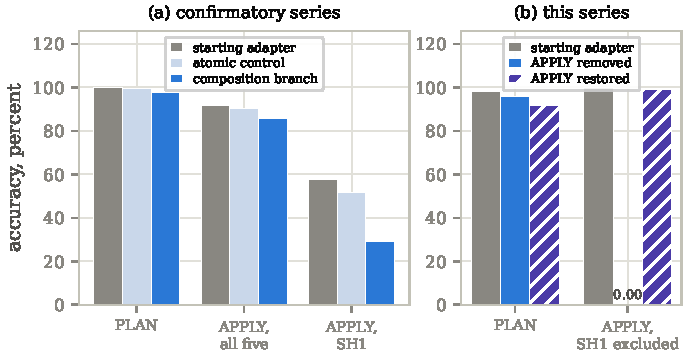
\includegraphics[width=0.95\textwidth]{pic/fig6_atomic.pdf}
    \caption{Retention of the atomic modes in the two series. The panels are not
    directly comparable: panel (a) averages APPLY over all five operations while panel
    (b) uses a split of the second series from which SH1 is excluded, and the two also
    differ in the training mixture.}
    \label{fig:atomic}
\end{figure}

\begin{figure}[!tbh]
    \centering
    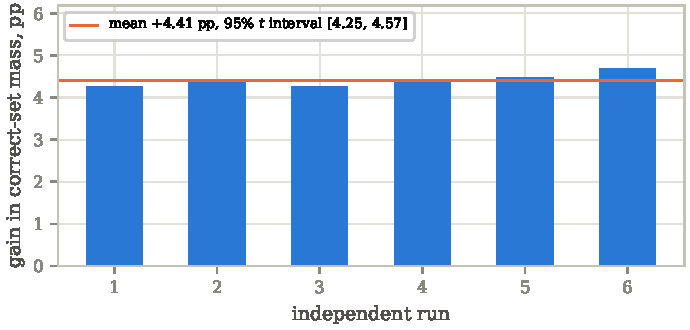
\includegraphics[width=0.95\textwidth]{pic/fig4_mass.pdf}
    \caption{Gain in the normalised probability mass of the correct set in each of the
    six independent runs, on the 1000 tasks of family A. The mean and the interval were
    recomputed from the six per-run values.}
    \label{fig:mass}
\end{figure}

\begin{figure}[!tbh]
    \centering
    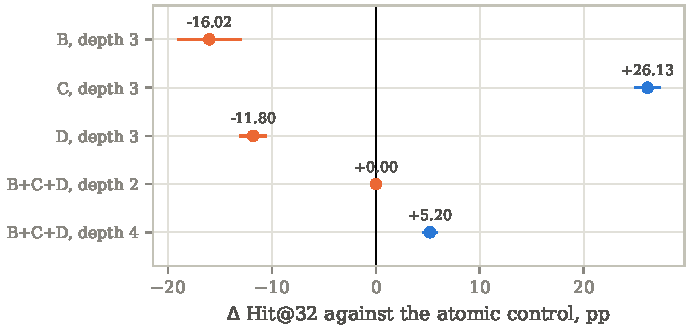
\includegraphics[width=0.95\textwidth]{pic/fig5_transfer.pdf}
    \caption{Secondary measures of transfer with their 95 percent intervals, as
    differences against the atomic control. Family B holds local motifs under
    familiar fields, C uses familiar signatures in new fields, and D combines the
    two. The depth-2 row is structurally saturated, so its zero carries no
    information. After the Holm correction the three depth-3 rows and the depth-4 row
    have $p$ values of $8.487 \times 10^{-5}$, $1.879 \times 10^{-7}$,
    $1.024 \times 10^{-5}$ and $2.976 \times 10^{-5}$.}
    \label{fig:transfer}
\end{figure}
% ------------------------------------------------- audit
\begin{table}[!tbh]
\centering\footnotesize\setlength{\tabcolsep}{6pt}
\begin{tabular}{|p{.52\linewidth}|l|}
\hline
\textbf{Check} & \textbf{Result} \\
\hline
six independent runs completed & yes \\ \hline
equality of the training budgets & confirmed \\ \hline
identical tasks for branches and runs & confirmed \\ \hline
number of leaks found & 0 \\ \hline
re-checked ranking shards & 2080 \\ \hline
completeness of the depth 2, 3 and 4 spaces & 25, 125 and 625 programs \\ \hline
re-check of labels and of the sort order & passed \\ \hline
preregistration created before the final data & yes \\ \hline
pilot adapters used in the confirmation & no \\ \hline
random generation at the main evaluation & not used \\ \hline
correction for multiple secondary tests & Holm \\ \hline
negative secondary results published & yes \\ \hline
\end{tabular}
\caption{Technical audit and reproducibility control of the confirmatory series. The
full re-check covered 2080 shard files of raw rankings, and for every task it
re-verified the completeness of the enumeration, the labels of the verifier and the
sort order.}
\label{tab:audit}
\end{table}


The full re-check covered 2080 shard files of rankings, verifying for every task the
completeness of the enumeration of 25, 125 or 625 programs, the correctness of the
labels and the sort order. The leak audit gave zero intersections, and the training
budgets inside each pair of branches were equal in optimiser steps, epochs, effective
batch size and loss-bearing target tokens. Acceleration on three RTX 5080 cards was
applied only to a part of the secondary rankings, and those data were reprocessed by
the frozen evaluation code. The compact audit archive publishes aggregated results and
the checksums of the 2080 shards, and not the individual rows of the main family-A
set for the composition branch, so no rank of an individual task of that set is
attributed anywhere in this paper.

\section{Full list of limitations}
\label{app:limits}

\begin{enumerate}
\item The study was carried out on one architecture and one model size. Transfer of
the result to other models requires separate verification.
\item The main positive result concerns familiar families of compositional
signatures on new inputs. Transfer to held local motifs is not confirmed.
\item The composition environment is synthetic. Its advantage is exact checking and
the complete enumeration of programs; real mathematical reasoning has a more complex
action space.
\item Atomic forgetting was substantial, especially for SH1. The method requires an
improved mechanism for preserving the base skills.
\item The number of independent runs of the confirmatory series equals six, which is
sufficient for the criteria fixed in advance, and the exact sign-permutation test has
a coarse resolution at that number of runs.
\item The second series uses three seeds and 300 tasks per split, which resolves a
contrast to roughly three percentage points. An interval containing zero means that
smaller effects would not have been detected.
\item Its self-training result covers one algorithm at one budget and one schedule.
It states that policy-gradient training under these conditions does not expand
coverage, and not that reinforcement learning cannot.
\item Three motifs were withheld out of the 25 adjacent pairs, the same three in both
series, and the size of the motif effect requires separate verification for the rest.
\item The verifier levels use one training seed each, and the boundary conditions of
Appendix~\ref{app:second} reuse evaluation sets that had already been opened. They
are reported as post-hoc controls.
\item The positive result should not be called the creation of a universal new
ability. It proves the consolidation and transfer of verified trajectories within a
clearly defined domain.
\end{enumerate}


\section{The second series}
\label{app:second}

\begin{figure}[!tbh]
    \centering
    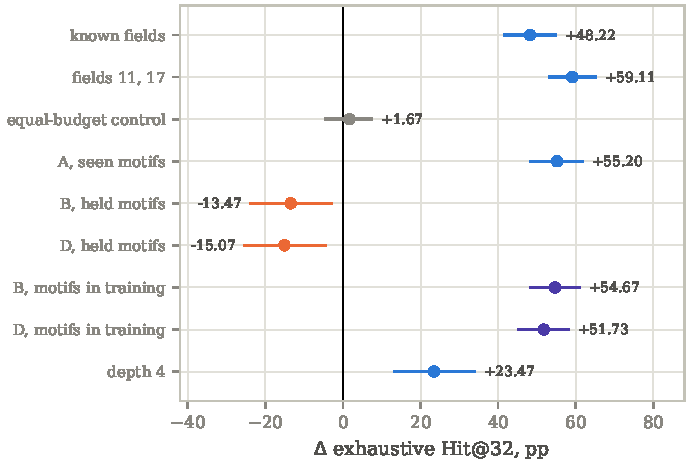
\includegraphics[width=0.95\textwidth]{pic/fig8_contrasts.pdf}
    \caption{Contrasts of the second series in exhaustive Hit@32 with their 95 percent
    crossed seed-by-task intervals. Rows in the darker colour are measured against the
    shared starting checkpoint, the grey row is an equal-budget atomic control, and the
    two rows in green are the same held-motif families ranked by adapters whose
    supervision contained the withheld pairs.}
    \label{fig:contrasts}
\end{figure}

The second series holds the same base model, the same operation set and the same
field division. It uses three training seeds, 300-task evaluation splits for the
depth and field grid and 250-task splits for the four motif families, and a 10000-fold
crossed seed-by-task bootstrap. Its supervised runs take 1875 optimiser steps at a
batch of 8 and a learning rate of $2 \times 10^{-4}$; its policy-gradient runs take 400
steps with a group size of 8, a learning rate of $1 \times 10^{-5}$ and a
Kullback-Leibler coefficient of 0.01. Its numbers are therefore not comparable with the
six-run intervals of the main text.

The two series also score programs differently: the confirmatory series reads the
log-probability of an operation off a softmax over the full vocabulary with five added
operation tokens, while the second series takes a softmax over the five admissible
continuations alone. Both rank by the same summed quantity, and the normaliser that the
first omits can reorder programs relative to the second, which bounds how literally
"reproduces" should be read across the two. An audit of the second series' ten splits
by exact key recorded overlaps in seven pairs, one of them a training-and-evaluation
leak of a single item; recomputed on never-trained items only the gate metrics are 1.00
on 72 items, 0.9775 on 89 and 0.8488 on 86, so the overlaps did not inflate them.

Studies E1 and E2 were preregistered in the ordinary sense. E3 was preregistered with
sampled pass@32 as its primary endpoint, and an amendment moved the primary weight to
exhaustive Hit@32; the sampled contrasts are $+63.33$ and $+62.56$ percentage points
against the exhaustive $+48.22$ and $+59.11$. E4, the motif axis, was added by that
same amendment, and its withheld set of three operation pairs was taken from the
confirmatory series after that series' own result was open, so E4 tests a hypothesis
chosen with knowledge of the effect on data generated independently of it. The
amendment file also carries a modification time about an hour after the last of E3's
primary ranking cells finished, so the order in which the amendment was written and
E3's data were read cannot be established from the artifacts. The boundary conditions
below reuse sets that E3 and E4 had already opened and are post-hoc throughout.

\begin{table}[!tbh]
\centering\scriptsize\setlength{\tabcolsep}{3pt}
\begin{tabular}{|l|p{.40\linewidth}|p{.19\linewidth}|l|}
\hline
& \textbf{Intervention} & \textbf{Evaluation} & \textbf{Status} \\
\hline
E1 & search method at matched candidate diversity & 300 tasks, 3 seeds & confirmatory \\ \hline
E2 & 400 steps of GRPO with an exploring sampler & 300 tasks, 3 seeds & confirmatory \\ \hline
E3 & supervision on correct depth-2 and depth-3 programs & $4 \times 300$, 3 seeds & confirmatory \\ \hline
E4 & removal of three operation pairs from supervision & $4 \times 250$, 3 seeds & confirmatory \\ \hline
E5 & equal-budget control, motif-present control, APPLY mixture, depth 4, verifier noise & reused sets, 125 new tasks & post-hoc \\ \hline
\end{tabular}
\caption{The five studies and their status, stated before any result is shown. E1
to E4 were preregistered, with the primary endpoint, the decision rule and the
frozen set fixed in advance. E4 was added by an amendment whose position in time
relative to the opening of E3's data cannot be established from the artifacts, so it
is a disclosed extension and not an independently preregistered test. E5 collects
boundary conditions on sets
that E3 and E4 had already opened, together with one newly generated depth-4
split, and is therefore reported as post-hoc. The verifier levels of E5 use one
training seed each and the rest of E5 uses three. The claims of E1 to E4 stand
without E5.}
\label{tab:design}
\end{table}

\begin{table}[!tbh]
\centering\footnotesize\setlength{\tabcolsep}{5pt}
\begin{tabular}{|l|r|r|}
\hline
\textbf{Search arm} & \textbf{pass@32} & \textbf{Distinct} \\
\hline
iid, $T=0.7$, the original control & 0.060 & 3.11 \\ \hline
iid, $T=1.6$ & 0.190 & 8.04 \\ \hline
iid, $T=2.0$ & 0.250 & 9.88 \\ \hline
iid, $T=3.0$ & 0.390 & 14.57 \\ \hline
iid, $T=5.0$ & 0.460 & 19.17 \\ \hline
iid, $T=8.0$ & 0.500 & 21.92 \\ \hline
iid, $T=100.0$, near uniform & 0.420 & 23.74 \\ \hline
temperature mixture & 0.090 & 4.25 \\ \hline
prefix-balanced, $T=0.7$ & 0.290 & 9.63 \\ \hline
\end{tabular}
\caption{Selection of the search arms on the development split at one seed: 100 PLAN
tasks over the fields 5 and 7, of which 46 are of depth two and 54 of depth three, so
the last column is an average over both depths. The last column counts distinct programs produced per task
inside a budget of 32 draws. Temperature here divides a summed sequence
log-probability, so these values are not comparable with ordinary decoding
temperatures. The arm at $T=2.0$ matches the realised diversity of prefix-balanced
search and fixes $T^{*}$, and the interior optimum at $T=8.0$ fixes the training
sampler of E2. No confirmatory set was opened for this selection.}
\label{tab:tempsweep}
\end{table}

\begin{table}[!tbh]
\centering\scriptsize\setlength{\tabcolsep}{4pt}
\begin{tabular}{|l|r|r|c|}
\hline
\textbf{Contrast} & \textbf{$\Delta$, pp} & \textbf{95\% CI} & \textbf{Seeds} \\
\hline
\multicolumn{4}{|l|}{E1, structure against diversity} \\ \hline
Q1, prefix-balanced $-$ iid at $T^{*}$ & $-1.11$ & $[-4.22, +1.89]$ & 0/3 \\ \hline
Q2, GRPO effect, iid branch & $-0.11$ & $[-0.89, +0.67]$ & 1/3 \\ \hline
Q2, GRPO effect, prefix branch & $-1.89$ & $[-3.78, +0.00]$ & 0/3 \\ \hline
Q3, the earlier diagonal, new set & $+9.00$ & $[+6.89, +11.11]$ & 3/3 \\ \hline
Q3, the earlier diagonal, earlier set & $+16.33$ & $[+13.17, +19.50]$ & 3/3 \\ \hline
Q4, iid at $T=3.0$ $-$ prefix-balanced & $+9.78$ & $[+6.44, +13.00]$ & 3/3 \\ \hline
\multicolumn{4}{|l|}{E2, self-training} \\ \hline
Q5, after GRPO $-$ its starting point & $+0.22$ & $[-3.11, +3.67]$ & 2/3 \\ \hline
Q6, exploring $-$ cold training sampler & $+0.89$ & $[-2.45, +4.22]$ & 2/3 \\ \hline
Q7, uniform random $-$ prefix-balanced & $+11.22$ & $[+7.33, +15.11]$ & 3/3 \\ \hline
Q8, best iid $-$ prefix-balanced & $+12.67$ & $[+8.89, +16.56]$ & 3/3 \\ \hline
\end{tabular}
\caption{Preregistered contrasts in sampled pass@32, three training seeds. The two
frozen exploration sets carry 300 depth-3 PLAN tasks each over fields 11 and 17; the
row marked as the earlier set is a third, earlier frozen set of 200 tasks, re-analysed
and not re-collected.
Intervals come from a 10{,}000-fold hierarchical paired bootstrap over tasks and
seeds. The last column counts the seeds whose own difference carries the sign of
the pooled estimate. Q1 and Q5 are the two primary endpoints, and both fall in the
preregistered branch where the interval contains zero.}
\label{tab:exploration}
\end{table}

\begin{table}[!tbh]
\centering\footnotesize\setlength{\tabcolsep}{4pt}
\begin{tabular}{|l|r|r|r|}
\hline
\textbf{Adapter} & \textbf{Accuracy} & \textbf{Distinct} & \textbf{pass@32} \\
\hline
before GRPO & 0.0151 & 3.80 & 0.044 \\ \hline
after GRPO, $T_{\text{train}}=0.7$ & 0.0139 & 2.49 & 0.038 \\ \hline
after GRPO, $T_{\text{train}}=8.0$ & 0.0358 & 1.81 & 0.061 \\ \hline
\end{tabular}
\caption{Decomposition of the null in Q5, measured at the search arm $T=0.7$ where
the preferences of the policy dominate the candidate set. Accuracy is the fraction
of drawn candidates the verifier accepts, and the third column counts distinct
programs per task inside a budget of 32 draws. The exploring policy is 2.37 times
more accurate per candidate and 2.10 times narrower.}
\label{tab:mechanism}
\end{table}

\begin{table}[!tbh]
\centering\scriptsize\setlength{\tabcolsep}{4pt}
\begin{tabular}{|l|r|r|}
\hline
\textbf{Contrast in exhaustive Hit@32} & \textbf{$\Delta$, pp} & \textbf{95\% CI} \\
\hline
\multicolumn{3}{|l|}{E3, against the shared starting checkpoint} \\ \hline
supervision, known fields & $+48.22$ & $[+41.33, +55.00]$ \\ \hline
supervision, fields 11 and 17 & $+59.11$ & $[+53.00, +65.33]$ \\ \hline
known $-$ held-out fields, after supervision & $-2.22$ & $[-6.00, +1.56]$ \\ \hline
depth 2 $-$ depth 3 at Hit@8, fields fixed & $+42.89$ & $[+38.00, +47.67]$ \\ \hline
\multicolumn{3}{|l|}{E5, against an equal-budget atomic control} \\ \hline
atomic control, known fields & $+0.11$ & $[-6.44, +6.44]$ \\ \hline
atomic control, fields 11 and 17 & $+1.67$ & $[-4.67, +7.67]$ \\ \hline
supervision $-$ atomic control, known fields & $+48.11$ & $[+38.67, +57.11]$ \\ \hline
supervision $-$ atomic control, fields 11, 17 & $+57.44$ & $[+49.67, +65.33]$ \\ \hline
\end{tabular}
\caption{Direct supervision on correct depth-3 programs, 300 tasks per split and
three training seeds, with all 125 candidate programs ranked exactly. The first two
rows of each block compare a trained adapter with the reference named in the block
heading. The atomic control received the same 1875 optimiser steps, the same
learning rate and the same number of training examples on atomic data alone, so
the lower block separates the content of the supervision from the length of the
optimisation.}
\label{tab:capacity}
\end{table}

\begin{table}[!tbh]
\centering\scriptsize\setlength{\tabcolsep}{4pt}
\begin{tabular}{|c|l|r|r|r|}
\hline
\textbf{Family} & \textbf{Fields, motifs} & \textbf{Hit@32} & \textbf{$\Delta$, pp} & \textbf{95\% CI} \\
\hline
\multicolumn{5}{|l|}{supervision with the three operation pairs withheld} \\ \hline
A & known, seen  & 0.940 & $+55.20$ & $[+48.13, +62.00]$ \\ \hline
B & known, held  & 0.253 & $-13.47$ & $[-24.00, -2.67]$ \\ \hline
C & 11 and 17, seen & 0.936 & $+58.80$ & $[+51.47, +65.73]$ \\ \hline
D & 11 and 17, held & 0.265 & $-15.07$ & $[-25.60, -4.27]$ \\ \hline
\multicolumn{5}{|l|}{supervision that contained those pairs} \\ \hline
B & known, held  & 0.935 & $+54.67$ & $[+48.13, +61.20]$ \\ \hline
D & 11 and 17, held & 0.933 & $+51.73$ & $[+45.07, +58.40]$ \\ \hline
\end{tabular}
\caption{The motif experiment, 250 depth-3 tasks per family and three training
seeds. A task enters a held family only when every minimal-depth correct program
for it contains one of the three withheld pairs, so an unheld route cannot solve
it. Differences are taken against the shared starting checkpoint, which reaches
Hit@32 of 0.388, 0.388, 0.348 and 0.416 on families A to D. The upper block is E4
and the lower block is the control of E5 on the same two evaluation families. The
motif main effect over the upper block is $+71.27$ pp, 95\% CI $[+58.53, +83.60]$,
and the field main effect is $-1.00$ pp, 95\% CI $[-8.27, +6.33]$.}
\label{tab:motif}
\end{table}

\begin{table}[!tbh]
\centering\scriptsize\setlength{\tabcolsep}{4pt}
\begin{tabular}{|p{.30\linewidth}|r|r|r|r|}
\hline
\textbf{Training mixture} & \textbf{APPLY} & \textbf{Parse} & \textbf{PLAN} & \textbf{Vectors} \\
\hline
no composition supervision & 1.000 & 1.000 & 0.980 & 80/80 \\ \hline
APPLY absent from the stream & 0.000 & 0.000 & 0.910--0.980 & 0/480 \\ \hline
APPLY at 17 percent of the stream & 0.975--1.000 & 1.000 & 0.850--0.970 & 240/240 \\ \hline
\end{tabular}
\caption{The atomic modes on the frozen validation splits, 80 APPLY tasks and 100
PLAN tasks, at greedy decoding. The APPLY and PLAN columns give pass@1 and the
Parse column gives the parse rate of the APPLY answers. The last column counts
answers to an APPLY prompt that contain a coefficient vector at all, pooled over
the six adapters of the middle row and the three of the last row.}
\label{tab:retention}
\end{table}

\begin{table}[!tbh]
\centering\footnotesize\setlength{\tabcolsep}{4pt}
\begin{tabular}{|l|r|r|r|r|}
\hline
\textbf{Adapter} & \textbf{Hit@1} & \textbf{Hit@8} & \textbf{Hit@32} & \textbf{Best rank} \\
\hline
no supervision & 0.000 & 0.016 & 0.056 & 237.6 \\ \hline
supervision, seed 0 & 0.040 & 0.128 & 0.336 & 92.8 \\ \hline
supervision, seed 1 & 0.024 & 0.104 & 0.336 & 88.9 \\ \hline
supervision, seed 2 & 0.016 & 0.072 & 0.200 & 143.2 \\ \hline
\end{tabular}
\caption{Exhaustive ranking of all 625 programs of depth~4 on 125 tasks over known
fields, where supervision had covered depths 2 and 3 only. The last column is the
mean rank of the best correct program. The pooled difference in Hit@32 is $+23.47$
pp, 95\% CI $[+13.07, +34.13]$, and the three seeds are listed separately because
they do not agree closely.}
\label{tab:depth4}
\end{table}


\begin{figure}[!tbh]
    \centering
    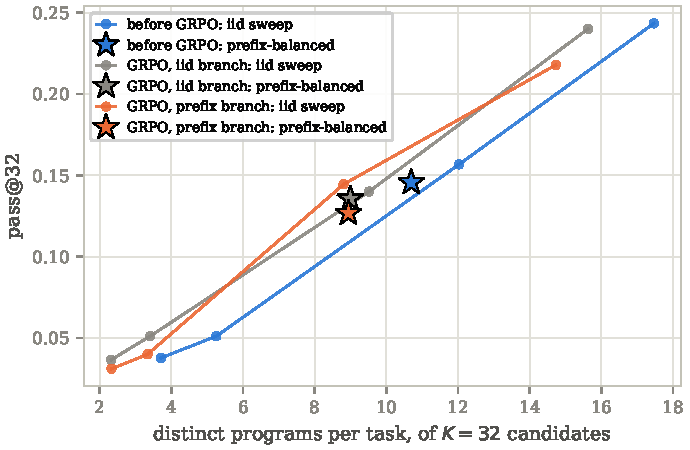
\includegraphics[width=0.95\textwidth]{pic/fig7_diversity.pdf}
    \caption{Coverage of the confirmatory set of the second series against realised
    candidate diversity, 300 depth-3 PLAN tasks over fields 11 and 17 at $K = 32$,
    averaged over three seeds. The stars, which mark prefix-balanced search, lie on
    the curve traced by the sweep over independent sampling temperatures.}
    \label{fig:diversity}
\end{figure}

\begin{figure}[!tbh]
    \centering
    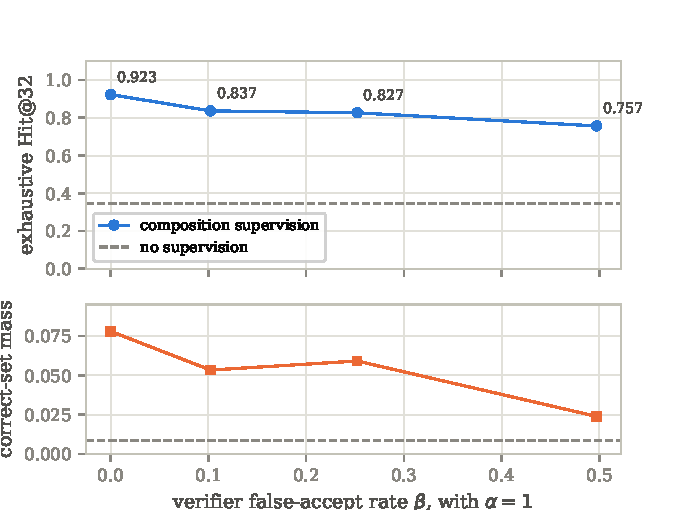
\includegraphics[width=0.95\textwidth]{pic/fig9_verifier.pdf}
    \caption{Composition supervision under a checking program that accepts every
    correct trajectory and a fraction $\beta$ of incorrect ones, on the 300 tasks of
    depth three over fields 11 and 17. One training seed per level, so this figure is
    exploratory and no interval over seeds is available.}
    \label{fig:verifier}
\end{figure}

\clearpage
\section*{References}
\providecommand{\bysame}{\leavevmode\hbox to3em{\hrulefill}\thinspace}
\providecommand{\MR}{\relax\ifhmode\unskip\space\fi MR }
\providecommand{\MRhref}[2]{%
  \href{http://www.ams.org/mathscinet-getitem?mr=#1}{#2}
}
\providecommand{\href}[2]{#2}
{\small\begin{thebibliography}{10}

\bibitem{chen2021codex}
Mark Chen, Jerry Tworek, Heewoo Jun, Qiming Yuan, Henrique~Ponde de~Oliveira
  Pinto, et~al., \emph{Evaluating large language models trained on code}, arXiv
  preprint arXiv:2107.03374, 2021.

\bibitem{cover2006information}
Thomas~M. Cover and Joy~A. Thomas, \emph{Elements of information theory},
  2nd ed., Wiley, 2006.

\bibitem{dziri2023faith}
Nouha Dziri, Ximing Lu, Melanie Sclar, Xiang~Lorraine Li, Liwei Jiang, et~al.,
  \emph{Faith and fate: Limits of transformers on compositionality}, Advances in
  Neural Information Processing Systems (NeurIPS), 2023.

\bibitem{efron1993bootstrap}
Bradley Efron and Robert~J. Tibshirani, \emph{An introduction to the bootstrap},
  Chapman and Hall, 1993.

\bibitem{gulcehre2023rest}
Caglar Gulcehre, Tom~Le Paine, Srivatsan Srinivasan, Ksenia Konyushkova,
  Lotte Weerts, et~al., \emph{Reinforced self-training ({ReST}) for language
  modeling}, arXiv preprint arXiv:2308.08998, 2023.

\bibitem{holm1979procedure}
Sture Holm, \emph{A simple sequentially rejective multiple test procedure},
  Scandinavian Journal of Statistics \textbf{6} (1979), no.~2, 65--70.

\bibitem{hu2022lora}
Edward~J. Hu, Yelong Shen, Phillip Wallis, Zeyuan Allen-Zhu, Yuanzhi Li,
  Shean Wang, Lu Wang, and Weizhu Chen, \emph{{LoRA}: Low-rank adaptation of
  large language models}, Proceedings of the International Conference on
  Learning Representations (ICLR), 2022.

\bibitem{kirkpatrick2017forgetting}
James Kirkpatrick, Razvan Pascanu, Neil Rabinowitz, Joel Veness,
  Guillaume Desjardins, et~al., \emph{Overcoming catastrophic forgetting in
  neural networks}, Proceedings of the National Academy of Sciences
  \textbf{114} (2017), no.~13, 3521--3526.

\bibitem{lake2018systematicity}
Brenden~M. Lake and Marco Baroni, \emph{Generalization without systematicity:
  On the compositional skills of sequence-to-sequence recurrent networks},
  Proceedings of the International Conference on Machine Learning (ICML), 2018,
  pp.~2873--2882.

\bibitem{lightman2024verify}
Hunter Lightman, Vineet Kosaraju, Yura Burda, Harrison Edwards, Bowen Baker,
  Teddy Lee, Jan Leike, John Schulman, Ilya Sutskever, and Karl Cobbe,
  \emph{Let's verify step by step}, Proceedings of the International Conference
  on Learning Representations (ICLR), 2024.

\bibitem{liu2025prorl}
Mingjie Liu, Shizhe Diao, Ximing Lu, Jian Hu, Xin Dong, Yejin Choi,
  Jan Kautz, and Yi Dong, \emph{{ProRL}: Prolonged reinforcement learning
  expands reasoning boundaries in large language models}, Advances in Neural
  Information Processing Systems (NeurIPS), 2025.

\bibitem{shao2024deepseekmath}
Zhihong Shao, Peiyi Wang, Qihao Zhu, Runxin Xu, Junxiao Song, Xiao Bi,
  Haowei Zhang, Mingchuan Zhang, Y.~K. Li, Y.~Wu, and Daya Guo,
  \emph{{DeepSeekMath}: Pushing the limits of mathematical reasoning in open
  language models}, arXiv preprint arXiv:2402.03300, 2024.

\bibitem{shumailov2024collapse}
Ilia Shumailov, Zakhar Shumaylov, Yiren Zhao, Nicolas Papernot,
  Ross Anderson, and Yarin Gal, \emph{{AI} models collapse when trained on
  recursively generated data}, Nature \textbf{631} (2024), 755--759.

\bibitem{wang2023selfconsistency}
Xuezhi Wang, Jason Wei, Dale Schuurmans, Quoc Le, Ed Chi, Sharan Narang,
  Aakanksha Chowdhery, and Denny Zhou, \emph{Self-consistency improves chain of
  thought reasoning in language models}, Proceedings of the International
  Conference on Learning Representations (ICLR), 2023.

\bibitem{yang2025qwen3}
An Yang, Anfeng Li, Baosong Yang, Beichen Zhang, Binyuan Hui, et~al.,
  \emph{{Qwen3} technical report}, arXiv preprint arXiv:2505.09388, 2025.

\bibitem{yao2023tot}
Shunyu Yao, Dian Yu, Jeffrey Zhao, Izhak Shafran, Thomas~L. Griffiths,
  Yuan Cao, and Karthik Narasimhan, \emph{Tree of thoughts: Deliberate problem
  solving with large language models}, Advances in Neural Information
  Processing Systems (NeurIPS), 2023.

\bibitem{yue2025rl}
Yang Yue, Zhiqi Chen, Rui Lu, Andrew Zhao, Zhaokai Wang, Yang Yue,
  Shiji Song, and Gao Huang, \emph{Does reinforcement learning really
  incentivize reasoning capacity in large language models beyond the base
  model?}, Advances in Neural Information Processing Systems (NeurIPS), 2025.

\bibitem{zelikman2022star}
Eric Zelikman, Yuhuai Wu, Jesse Mu, and Noah~D. Goodman, \emph{{STaR}:
  Bootstrapping reasoning with reasoning}, Advances in Neural Information
  Processing Systems (NeurIPS), 2022.

\bibitem{zhao2024skill}
Haoyu Zhao, Simran Kaur, Dingli Yu, Anirudh Goyal, and Sanjeev Arora,
  \emph{Can models learn skill composition from examples?}, Advances in Neural
  Information Processing Systems (NeurIPS), 2024.

\end{thebibliography}

}

\end{document}
